\section{Method}
Our method is strictly borrowed from Caldarelli et al. \cite{caldarelli2012network}. We investigate the properties of the biased Markov chains formulation of the {\it reflexion method}, in the slightly different context of open collaboration. In this specific context, the bi-partite network has two types of nodes : the editors (i.e., the producing entities) and the articles (i.e. the products). While the method is unchanged, the nature of the input (i.e. the description of the bi-partite network) as well as the interpretation of the relationships are different. Specifically, editors are not competing for the production of an article. They rather cooperate, implicitly according to the rules of peer-production or explicitly through the discussion page attached to each article, in order to increase the quality of the article.

The simplest way to represent a bi-partite network of online collaboration is to consider that an editor is linked to an article when she has ever made a modification. The resulting input of our model is a binary matrix $\mathbf{M}$ of editors and the articles they have modified as shown on Figure \ref{fig:matrix}. 

\begin{figure*}[!t]
\centering
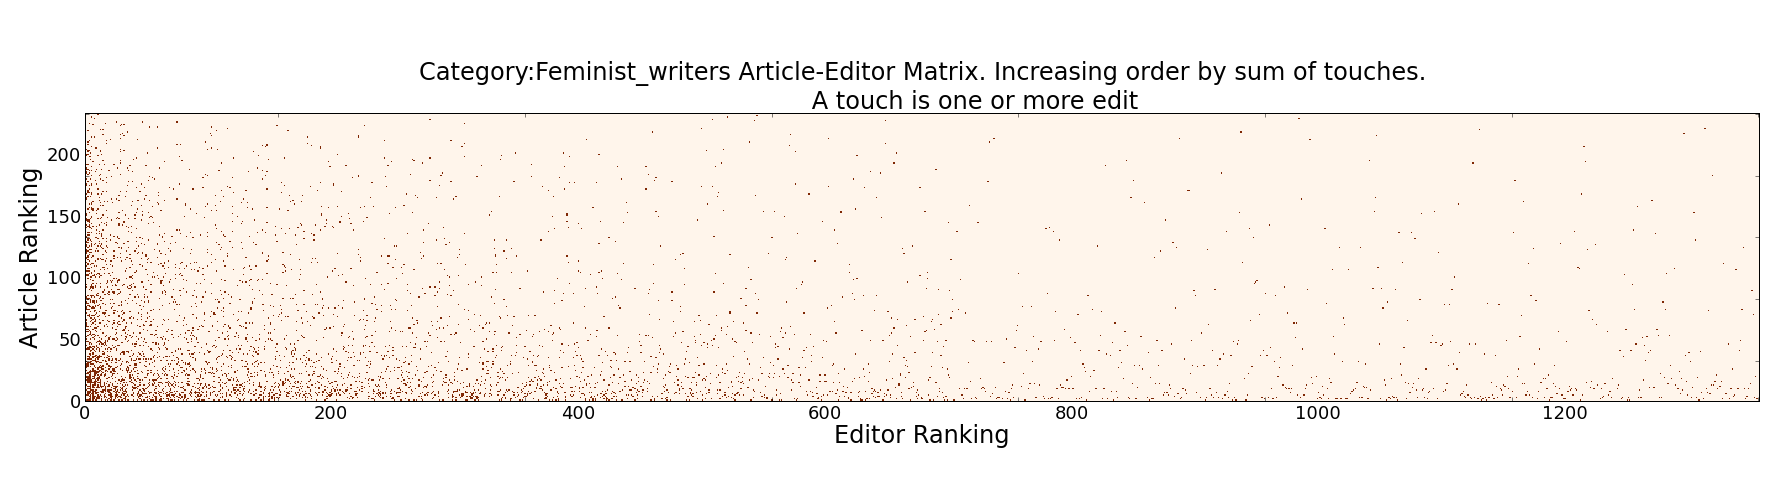
\includegraphics[width=2.0\columnwidth]{Figures/Category_Feminist_writerstriangle_matrix_corrected.png}
\caption{Typical $\mathbf{M}$ matrix for a Wikipedia category (here, {\it Feminist Writers}) ordered on both dimensions by descending order of number of articles modified by an editor (horizontal axis) and of number editors who have modified an article (vertical axis). The structure of $\mathbf{M}$ is triangular and shows that some editors have a pervasive activity over articles, while most editors edit only a few. Similarly, some articles receive widespread attention by editors, while most articles are modified only by a few editors.}
\label{fig:matrix}
\end{figure*}


The matrix $\mathbf{M}$ shown in Figure \ref{fig:triangle_matrix} shows when an article has changed at some point by a given editor. The matrix is ordered on both dimensions by decreasing order of editors who have changed more articles (vertical axis) and by decreasing order of articles that have been changed by most editors (horizontal axis) for a category of Wikipedia articles (here Feminist Writers). Although it is a rough count, the matrix tells already about the experience of an editor in the given category, and the attention an article has gotten from editors, which is an implicit quality measure according to the second principle of peer-production : peer-review. This count is the zero order of the Article/Editor ranking algorithm, and thus the initiation step is given by 

When ordered on both dimensions by decreasing order of editors who have changed more articles (vertical axis) and by decreasing order of articles that have been changed by most editors (horizontal axis), the matrix $\mathbf{M}$ exhibits a triangular structure, which is at odds with the traditionally accepted idea that editors tend to specialize \cite{}. In that later case, $\mathbf{M}$ should rather be diagonal. On the contrary, some editors have a pervasive activity over all articles, while most editors edit only a few. Similarly, some articles receive widespread attention by editors, while most articles are modified only by a few editors. The matrix $\mathbf{M}$ gives also immediate information on the zero\textsuperscript{th} iteration of the reflexion method: the number of articles modified (horizontal axis) gives information on the expertise of the editor, while the number of editors who have modified an article give an information on the quality of the article : one of the fundamental rules of open source development is that {\it ``Given enough eyeballs, all bugs shallow"} \cite{raymond1999}. The initiation step of the reflexive algorithm is therefore given by,

\begin{equation}
\begin{cases}
 \mathbf{d}_{e}^{(0)} = \sum_{a=1}^{N_{a}} \mathbf{M}_{ea} \equiv \mathbf{k}_e\\
 \mathbf{u}_{a}^{(0)} = \sum_{e=1}^{N_{e}} \mathbf{M}_{ea}  \equiv \mathbf{k}_a.\\
\end{cases}
\label{HHinit}
\end{equation}

The principal argument for going to further steps is following : the zero\textsuperscript{th} is quite rough: the number of articles modified tells actually little on expertise of editors because we don't know the value of the modified articles. Similarly the number of editors tells little about the quality of an article because the expertise of the editors who have modified the article is unknown. The second step of the algorithm is therefore the following: if an article has been changed by editors who edited more articles, then the quality of the article should be higher. Similarly, if an editor has edited articles that have been edited by more editors, then the expertise of the editor should be higher {\bf [(the only reason for making this claim is the collaborative nature of Wikipedia, and learning by imitation)]}.  Accordingly, the third step is the following : if an article has been changed by editors who edited more articles, which in turn have been edited by more editors, then the quality of the article should be higher. Similarly, if an editor has edited articles that have been edited by more editors, who in turn have edited more articles, then the expertise of the editor should be higher. The algorithm goes on recursively, incorporating the quality (resp. expertise) information of the article (resp. editor) at the previous step. The way the iterative step was initially formulated is the following, 

\begin{equation}
\begin{cases}
 \mathbf{d}_{e}^{(n+1)} = \frac{1}{\mathbf{k}_a} \sum_{a=1}^{N_{a}} \mathbf{M}_{ea} \mathbf{u}_{a}^{(n)}\\
 \mathbf{u}_{a}^{(n+1)} = \frac{1}{\mathbf{k}_e}\sum_{e=1}^{N_{e}} \mathbf{M}_{ea} \mathbf{d}_{e}^{(n)}\\
\end{cases}
\label{HHalgo}
\end{equation}

where $d_{e}$ stands for diversification of editors and $u_{a}$ for the ubiquity of articles.

{\bf While it is following very well the intuition behind the algorithm, ``The major problem of this formulation is that it is a case of consensus dynamics \cite{shamma2007cooperative}, i.e. the state of a node at iteration t is just the average of the state of its neighbors at iteration t-1".[ reformulate] } This approach converges rapidly to a fixed point, which is undesirable if the goal is precisely to discriminate as best as possible between editors and articles. The idea of Caldarelli et al. \cite{caldarelli2012network} is to treat the problem as a problem of a {\it random walker} jumping from one node to another along the edges of the bi-partite network. In other words, the random walker jumps with some probability from an editor to a linked article, or from an article to a linked editor. The weights of vertices are proportional to the time spent by the random walker in the large time limit \cite{zlatic2010}.  The intuition is that an editor (resp. an article) with more links from articles (resp. from editors) has more chances to be visited by the random walker. However, if the random walker is unbiased, the algorithm is not different from the zero\textsuperscript{th} order of the reflections method given by (\ref{HHinit}). Therefore, some biases $\alpha$ (resp. $\beta$) on the probability to jump from an article to an editor (resp. from an editor to an article). Such weights are the generalization of $k_e$ and $k_a$, and give a measure of editors' expertise and of articles' quality. At the $n$\textsuperscript{th} step, the algorithm writes,

\begin{equation}
\begin{cases}
 \mathbf{w}^{(n+1)}_e (\alpha,\beta) = \sum_{p=1}^{N_a}  \mathbf{G}_{cp}(\beta) \mathbf{w}^{(n)}_a (\alpha,\beta)\\
\mathbf{w}^{(n+1)}_a (\alpha,\beta) = \sum_{c=1}^{N_e}  \mathbf{G}_{pc}(\beta) \mathbf{w}^{(n)}_e (\alpha,\beta),\\
\end{cases}
\label{random_walker}
\end{equation}

with the Markov transition matrices $\mathbf{G}_{ea}(\beta)$ and $\mathbf{G}_{ae}(\alpha)$ control the biased of the random walk and are given by 

\begin{equation}
\begin{cases}
\mathbf{G}_{ea}(\beta) = \frac{\mathbf{M}_{ea} \mathbf{k}_{e}^{-\beta}}{\sum_{e' = 1}^{N_e} \mathbf{M}_{e'a} \mathbf{k}_{e'}^{-\beta}}\\
\mathbf{G}_{ae}(\alpha) = \frac{\mathbf{M}_{ea} \mathbf{k}_{a}^{-\beta}}{\sum_{a' = 1}^{N_a} \mathbf{M}_{e'a} \mathbf{k}_{a'}^{-\beta}}\\
 \end{cases}
\end{equation}

{\bf with $c'$ and $p'$ are XXX [to be completed]} Here $G_{ea}$ gives the probability to jump from article $a$ to editor $e$ in a single step, and $G_{ae}$ the probability to jump from editor $e$ to article $a$ also in a single step. We shall give more insights on how $\alpha$ and $\beta$ influence the random walker by analyzing the transition matrices $\mathbf{G}_{ea}(\beta)$ and $\mathbf{G}_{ae}(\alpha)$. The transition matrices depend only from the initial conditions $\mathbf{M}$ and $k_e$ and $k_a$ given by (\ref{HHinit}). Since both transition matrices have the same structure, we only consider $\alpha$  and $\mathbf{G}_{ae}(\alpha)$. $\alpha$ is the power exponent of the inverse of $k_a$, and therefore the bias depends on the possible values taken by $\alpha$. If $\alpha = 0$, we recover the zero\textsuperscript{th}. For $\alpha > 0$, the probability to jump is weighted by a concave function of the sum of editors who have modified the article. The larger $\alpha$ the less the number of editors is important to an article. On the contrary, if $\alpha < 0$ the probability to jump from an editor to an article is a positive function of the sum of editors who have modified the article. For $-1 < \alpha < 0$, the function is concave, while for $\alpha < -1$, the function is convex, which means that the more editors, the even more the weight on the article. The same considerations hold for $\beta$ and the probability $\mathbf{G}_{ea}$ to jump from an article to an editor. 



A ranking-by-iteration plot shows how the ranking typically converges over iterations. As shown in Figure \ref{fig:convergence}, the algorithm converges in a non-trivial way, they can be reduced ergodic Markov chains \cite{Firm Grounds}. In the iterative solution we see how certain editors start low, but then climb in rankings. This means that they are editing few articles, but those articles are of higher quality. Likewise certain articles climb over iterations, they are edited by relatively few editors, but those editors are fitter.

where $c'$ and $p'$ are :

Here $G_{cp}$ gives the probability to jump from product p to country c
in a single step, and $G_{pc}$ the probability to jump from country $c$ to
product $p$ also in a single step.


The random walkers starting from editors jump on articles at odd steps, and back on editors from article at even steps. Figure \ref{} shows how the ranking typically converges over iterations. As shown on Figure \ref{fig:convergence}, the algorithm converges in a non-trivial way {\bf (explanation for this?)}. In the iterative solution we see how certain editors start low, but then climb in rankings. This means that they are editing few articles, but those articles are of higher quality. Likewise certain articles climb over iterations, they are edited by relatively few editors, but those editors are fitter.


With the following balance condition,

\begin{equation}
\mathbf{G}_{pc} \mathbf{w}^*_c = \mathbf{G}_{cp} \mathbf{w}^*_p
\end{equation}

An analytical solution can be found \cite{caldarelli}

\begin{equation}
\begin{cases}
 w^*_c = A(\sum^{N_p}_{p=1} M_{cp}k_p^{-\alpha})k_c^{-\beta} \\
w^*_p = B(\sum^{N_c}_{c=1} M_{cp}k_c^{-\beta})k_p^{-\alpha}
\end{cases}
\end{equation}



\begin{figure}[!t]
\centering
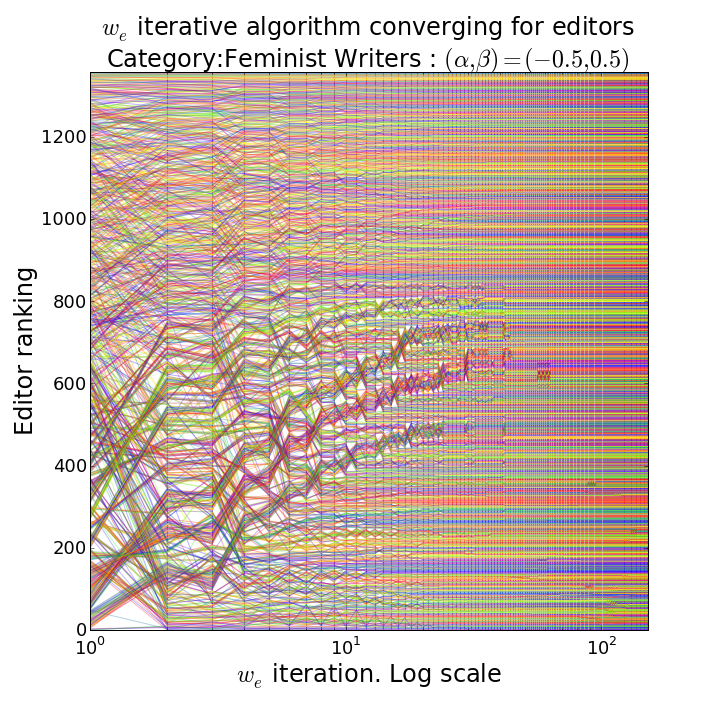
\includegraphics[width=0.9\columnwidth]{Figures/fem_editors_iter_converge.png}.
\caption{Typical evolution of the editors' ranking as a function of iterations of the biased random walker as  given by (\ref{random_walker}) with biases $\alpha = -0.5$ and $\beta = 0.5$ for the Wikipedia category \textit{\textbf{ Feminist Writers}}. The higher rank the higher the expertise of the editor. The algorithm nearly converges to stable ranks after a hundred iterations.}
\label{fig:convergence}
\end{figure}

If the balance condition $\mathbf{G}_{pc} \mathbf{w}^*_e = \mathbf{G}_{cp} \mathbf{w}^*_a$
%\begin{equation}
%\mathbf{G}_{pc} \mathbf{w}^*_e = \mathbf{G}_{cp} \mathbf{w}^*_a
%\end{equation}
is applied, an analytical solution can be derived \cite{caldarelli}, which is given by,

\begin{equation}
\begin{cases}
 \mathbf{w}^*_e \sim (\sum^{N_a}_{p=1} \mathbf{M}_{cp} \mathbf{k}_a^{-\alpha}) \mathbf{k}_e^{-\beta} \\
\mathbf{w}^*_a \sim (\sum^{N_e}_{c=1} \mathbf{M}_{cp} \mathbf{k}_e^{-\beta}) \mathbf{k}_a^{-\alpha},
\end{cases}
\end{equation}

%\begin{figure}[!t]
%\centering
%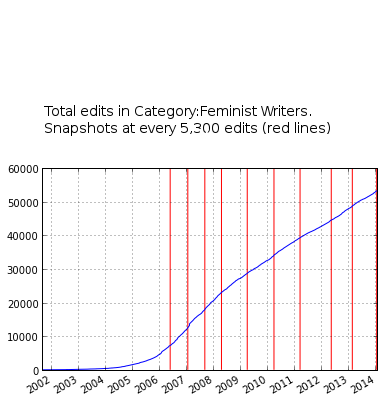
\includegraphics[width=0.9\columnwidth]{Figures/accumulative snapshot points for Feminist Writers.png}
%\caption{Convergence}
%\label{fig:convergence}
%\end{figure}

that we use onwards. It is important to note a crucial difference in the way we apply the weighted random walk model in the case of open collaboration compared to the countries-products problem. In \cite{caldarelli2012network}, $w^*_p$ is a measure of ubiquity (i.e. dis-quality) because many countries can sell the product, while here $w^*_a$ is also a measure of ubiquity in the sense that many editors have modified the article. In the case of open collaboration, $w^*_a$ is a measure of quality.

Our aim here is to calibrate $\alpha$ and $\beta$ for various categories of articles on Wikipedia against some exogenous metrics of editors' expertise and articles' quality, to understand how the biases can inform on the emergence of respectively expertise and quality.
